\documentclass[border=4pt]{standalone}
\usepackage{tikz}
\usetikzlibrary{shapes.symbols,positioning}

\begin{document}
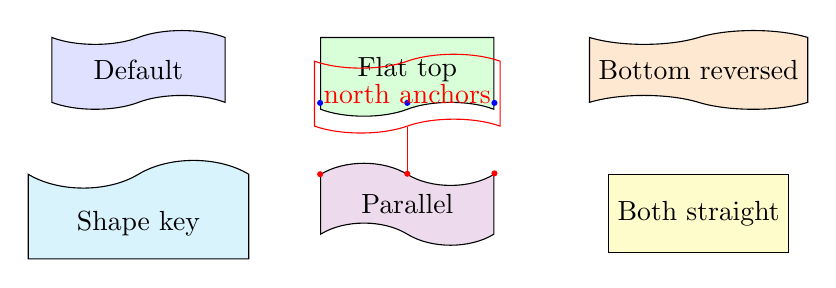
\begin{tikzpicture}[
  every node/.style={tape,draw,minimum width=22mm,minimum height=10mm,align=center},
  node distance=9mm and 12mm
]
  \node[fill=blue!12] (default) {Default};
  \node[tape bend top=none,fill=green!15,right=of default] (flat) {Flat top};
  \fill[blue] (flat.south west) circle (1.1pt);
  \fill[blue] (flat.south) circle (1.1pt);
  \fill[blue] (flat.south east) circle (1.1pt);
  \node[tape bend bottom=out and in,fill=orange!18,right=of flat] (reverse) {Bottom reversed};

  \node[tape bend=out and in,tape bend height=8pt,fill=violet!14,
    below=of flat] (parallel) {Parallel};
  \fill[red] (parallel.north west) circle (1.1pt);
  \fill[red] (parallel.north) circle (1.1pt);
  \fill[red] (parallel.north east) circle (1.1pt);
  \draw[red,thin] (parallel.north) -- ++(0,6mm) node[above]{north anchors};

  \node[shape=tape,tape bend bottom=none,tape bend height=10pt,
    minimum width=28mm,fill=cyan!15,below=of default] (bottomflat) {Shape key};
  \node[tape bend top=none,tape bend bottom=none,fill=yellow!20,
    below=of reverse] (plain) {Both straight};
\end{tikzpicture}
\end{document}
